
\section{Optimal joint assignment (OJA)}\label{sec:qp}

Since heatmaps generated by the joint predictor are multi-modal, the non-maximum suppression procedure yields multiple possible locations for each joint. The set of joint proposals is represented as $X = \{x_{jp}\}$, where $x_{jp}$ indicates the 2D position of proposal $p \in \{1,...,N_j\}$ associated with joint $j \in J$.
Before applying the optimizer, a subset of proposals $X^* \subseteq X$ should be selected in order to form a complete skeleton, i.e. precisely \emph{one proposal is selected for every joint}. This section will consider how to choose the optimal subset by formulating the problem as an extended optimal assignment problem.

In order to select a complete skeleton proposal from the set of joint proposals $\{x_{jp}\}$, a binary indicator vector $\bvec a_j = \{a_{jp}\} \in \{0, 1\}^{N_j+1}$ is introduced, where $a_{jp} = 1$ indicates that the $p^\text{th}$ proposal for joint $j$ is a correct assignment, and the $p = N_j+1$ position corresponds to a {\em null proposal}, indicating that joint $j$ has no match in this image.
The null proposals are handled as described in each of the energy terms below.
Let $A$ be the jagged array $[\bvec a_j]_{j=1}^J$ containing all assignment variables (for the current frame), and let $X^* = X(A)$ denote the subset of points selected by the binary array $A$.


% Please add the following required packages to your document preamble:
% \usepackage{booktabs}
% \usepackage{multirow}
\begin{table}
    \RawFloats
    \parbox{.48\linewidth}{
        \strut
        \centering
        \begin{tabular}{@{}llll@{}}
        \toprule
        Joint $j$               & Proposal $p$ & $x_{jp}$ & $a_{jp}$ \\ 
        \midrule
        \multirow{3}{*}{Nose} & 0          & $(0, 2) $   & 1 \\
                            & 1          & $(4, 2) $   & 0 \\
                            & NULL       & ---         & 0 \\
        \midrule
        Upper Leg             & NULL       & ---         & 1 \\
        \midrule
        \multirow{3}{*}{Paw}  & 0          & $(4, 2)$    & 0 \\
                            & 1          & $(8, 10)$   & 1 \\
                            & NULL       & ---         & 0 \\
        \midrule
        \multirow{4}{*}{Tail} & 0          & $(4, 2)$    & 0 \\
                            & 1          & $(8, 10)$   & 0 \\
                            & 2          & $(4, 2)$    & 1 \\
                            & NULL       & ---         & 0 \\
        \bottomrule
        \end{tabular}
        \caption{Example inputs and output to the joint assignment problem. Non maximum suppression applied to predicted heatmap tensors yields a set of proposals $p$ for each each skeleton joint $j$ at 2D location $x_{jp}$. $a_{jp}$ is an illustrative assignment vector which is predicted by the OJA algorithm.}
        \label{tab:oja-example-inputs}
    }
    \hfill
    \parbox{.48\linewidth}{
        \strut
        \centering
        \parbox{\linewidth}{
            \strut
            \centering
            \begin{tabular}{@{}lllll@{}}
            \toprule
            Joint $j$ & \multicolumn{4}{l}{Proposal $p$}                                                 \\
            \midrule
            Nose      & 1 & 0                        & 0                        & \cellcolor[HTML]{808080} \\
            Upper Leg & 1 & \cellcolor[HTML]{808080} & \cellcolor[HTML]{808080} & \cellcolor[HTML]{808080} \\
            Paw       & 0 & 1                        & 0                        & \cellcolor[HTML]{808080} \\
            Tail      & 0 & 0                        & 1                        & 0                        \\
            \bottomrule
            \end{tabular}
            \caption{Assignment variables $A = \bvec a_j = \{a_{jp}\} \in \{0, 1\}^{N_j+1}$ for the current frame stored as a jagged array.}
            \label{tab:oja-proposals}
        }
        \bigskip
        \parbox{\linewidth}{
            \strut
            \centering
            \begin{tabular}{@{}ll@{}}
                \toprule
                Joint $j$ & $X^* = X(A)$ \\
                \midrule
                Nose      & $(0, 2)$     \\
                Upper Leg & ---          \\
                Paw       & $(8, 10)$    \\
                Tail      & $(4, 2)$     \\
                \bottomrule
            \end{tabular}
            \caption{2D joint locations $X^* = X(A)$ selected by the assignment variable $A$}
            \label{tab:oja-selected}
        }
    }
\end{table}        
        

Optimal assignment minimizes the function
\begin{equation}
L(A) = \LL{conf}(A) + \LL{null}(A) + \LL{prior}(A) + \LL{temp}(A) + \LL{cov-sil}(A) + \LL{cov-bone}(A)
\end{equation}
which balances agreement of the joint configuration with the network-supplied {\em confidences}, a learned {\em prior}, {\em temporal} coherence, and {\em coverage} terms which encourage the model to correctly project over the silhouette. Without the coverage terms, this can be optimized as a quadratic program, but better results are obtained by including the coverage terms, and using a genetic algorithm. In addition, the parameters $A$ must satisfy the $J$ constraints $\sum_{p=1}^{N_j+1} a_{jp} = 1$, that exactly one joint proposal (or the null proposal) must be selected for each joint.

\subsection{Basic formulation}

\subsubsection{Network confidences: $\LL{conf}(A)$}

The first energy term $\LL{conf}(A)$ comes from the output of the joint prediction network, which provides a confidence score $y_{jp}$ associated with each joint proposal~$x_{jp}$.  Then $\LL{conf}(A) = \sum_j\sum_p -\lambda_{\text{conf}}\log(y_{jp}) A_{jp}$ is a linear function of $A$, 
and $\lambda_{\text{conf}}$ is a tunable parameter to control the relative contribution of the network confidences compared with that of the skeleton prior. Note that if only this term is included, the OJA would simply produce the result of the standard non-maximal suppresion algorithm, selecting the heatmap location with highest network confidence. Note that this function can be rewritten as

\begin{equation}\label{eq:conf-energy}
    \LL{conf}(A) = \lambda_{\text{conf}}\log(y^T) \text{vec}(A)
\end{equation}

\subsubsection{Null proposals: $\LL{null}(A)$}

Under some circumstances, for example when a body part is heavily occluded or ambiguous, \emph{all} available proposals for a given joint may be of poor quality. In such a case, including any of these options in a skeleton configuration may have a detrimental impact on the later model fitting stage. Under these circumstances, it may be preferable to exclude the joint in question from the optimization entirely. Null proposals pay a fixed cost $\lambda_{null}$, effectively acting as a threshold whereby the null proposal will be selected if no other proposal is of sufficient likelihood. Precisely, a jagged array $D$ is defined

\begin{equation}
    D_{jp} = \begin{cases}
        \lambda_{\text{null}} & \text{if } p \text{ is null proposal}\\
        0 & \text{otherwise}
    \end{cases}
\end{equation}

and resulting energy becomes

\begin{equation}\label{eq:null-energy}
    \LL{null}(A) = \text{vec}(D) \text{vec}(A)
\end{equation}

\subsubsection{Skeleton Prior: $\LL{prior}(A)$}

The next energy term is used to discourage anatomically implausible skeletal configurations from being selected. The prior probability of a skeletal assignment $A$ is represented as a multivariate Gaussian distribution over the selected joint positions $X^* = X(A)$

% % Here, x is used as a general 2D coordinate
\begin{equation}
P_{\mathrm{prior}}(A) = \frac{1}{\sqrt[]{(2\pi)^k\left|\Sigma\right|}}\exp\left(-\frac{1}{2}(x^*-\mu)^T\Sigma^{-1}(x^*-\mu)\right)
\end{equation}

The mean $\mu \in \R{2J}$ and covariance $\Sigma \in \R{2J\times 2J}$ terms are obtained from synthetic training examples generated earlier. The prior is shown in \Cref{fig:skeleton-prior}. The objective of the OJA is to find the assignment vector $A$ which maximizes this prior, which is equivalent to minimizing the negative log prior
\begin{equation}
    \LL{prior}(A) = \frac{k}{2}\log(2\pi) + \frac{1}{2}\left|\Sigma\right| + \frac{1}{2}(x^*-\mu)^T\Sigma^{-1}(x^*-\mu)
\end{equation}

This formulation is reducible to a minimization over the Mahalanobis distance, which is given by the summation
\begin{equation}
\LL{prior}(A) = \sum_j^J\sum_p^{N_j}\sum_k^J\sum_q^{N_k}a_{jp}a_{kq}(x_{jp} - \mu_j)\Sigma_{jk}^{-1}(x_{kq}-\mu_k)
\end{equation}

Notice this is a quadratic function of $A$, so $\LL{prior}(A) = \text{vec}(A)^\top Q \text{vec}(A)$ for a fixed matrix $Q$. Precisely, the elements of the matrix $Q$ are precisely the Mahalanobis distance between each individual pair of joint proposals
\begin{equation}
\left[Q\right]_{jp, kq} = (x_{jp} - \mu_j)\Sigma_{jk}^{-1}(x_{kq}-\mu_k)
\end{equation}

Null proposals are simply excluded from the sum, equivalent to marginalizing over their position. 


\begin{figure}[t]
\def\bb{\rule{2in}{0pt}\rule{0pt}{1in}}
\begin{tabular}{cccc}
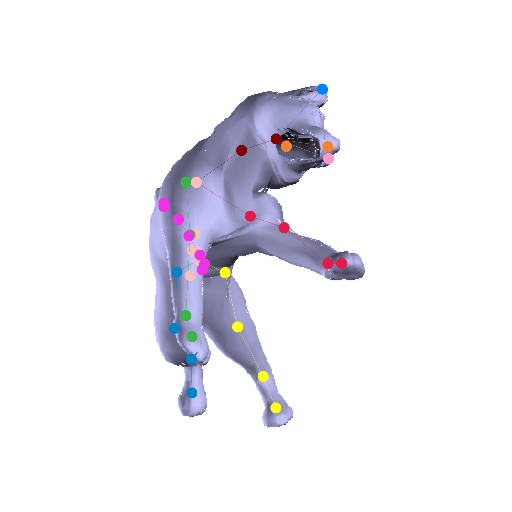
\includegraphics[width=0.25\linewidth]{skeletal_prior_gen/63_rgb.png} & 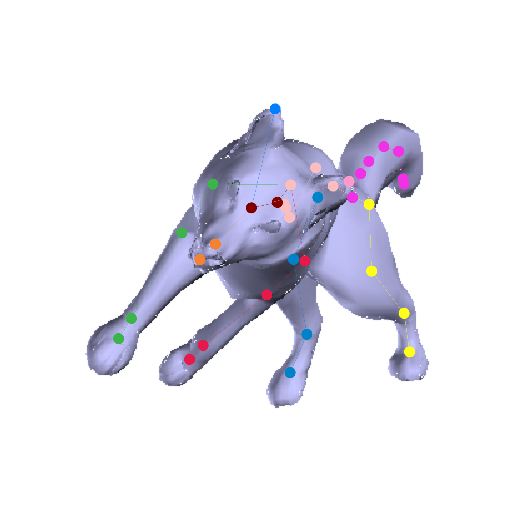
\includegraphics[width=0.25\linewidth]{skeletal_prior_gen/36_rgb.png} & 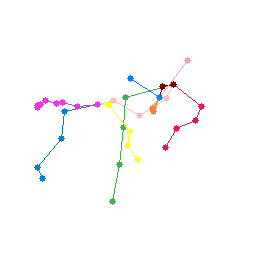
\includegraphics[width=0.25\linewidth]{skeletal_prior/74.png} & 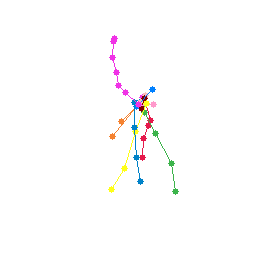
\includegraphics[width=0.25\linewidth]{skeletal_prior/108.png} \\
(a) & (b) & (c) & (d) \\
\end{tabular}
\caption{Skeleton Prior: Synthetic quadruped training data examples (rendered with texture to show 3D) generated by sampling pose, shape and position parameters and applying to SMAL model (a), (b). The set of 2D skeletal positions are used to create a vector of means $\mu \in \mathbb{R}^{2J}$ and covariance matrix $\Sigma \in \mathbb{R}^{2J \times 2J}$. The Gaussian distribution constructed can be sampled to create new skeletons, such as those shown in (c), (d).}
\label{fig:skeleton-prior}
\end{figure} 

\subsubsection{Temporal Prior: $\LL{temp}(A)$}
% TODO: Consider bringing in qp_defs/IMAGES to help explain and draw matrices Q
A common failure case of the joint prediction network is in situations where a joint position is highly ambiguous, for example between the left and right legs. In such cases, the algorithm will commonly alternate between two equally likely predictions. This leads to large displacements in joint positions between consecutive frames which are difficult for the later model fitting stage to recover from. This can be addressed by introducing a temporal term into the OJA. A prior is imposed on the distance moved by each joint between frame $t_0$ and $t_1$, which is given by a normal distribution with zero mean and variance $\sigma^{2} =e^{\tau|t_1 - t_0 - 1|}$. 
The parameter $\tau$ controls the strength of the interaction between distant frames. This results in an additional quadratic term in our objective function, which has the form $L_{temp} = a^\top T^{(t_0, t_1)} a$ for matrix $T^{(t_0, t_1)}$ given by 
\begin{equation}
\left[T^{(t_0, t_1)}\right]_{jp, kq} = \begin{cases}
e^{-\alpha|t_1 - t_0 - 1|}||x^{(t_0)}_{jp} - x^{(t_1)}_{kq}||^2 & \text{if } j=k\\
0 & \text{otherwise}
\end{cases}
\end{equation}

\subsection{QP solution.}
A general quadratic program is made up of a quadratic objective function and linear equality and inequality constraints. Thus far, all terms in $L(A)$ are quadratic or linear. 

To optimize over a sequence of frames, we construct the block diagonal matrix $\hat{Q}$ whose diagonal elements are the prior matrices $Q^{(t)}$ and off-diagonal elements are the temporal matrices $T^{(t_0, t_1)}$. The confidence term \Cref{eq:conf-energy} and null penalty term \Cref{eq:null-energy} are combined and the vector $\hat{c}$ is obtained by stacking across each frame. The solution vector for the sequence $\hat{a}$ is similarly constructed by stacking the vectorized assignment matrices $A$ across timesteps. The jagged array $B$ is used to formalize the constraint that only one proposal should be selected per joint. Precisely

\begin{equation}
    \left[B\right]_{jp,kq} = \begin{cases}
        1 & \text{if } j=k\\
        0 & \text{otherwise}
    \end{cases}
\end{equation}
and (similarly to $A$) is vectorized and stacked across timesteps to form the constraint $\hat{B}\hat{a} = 1$. Finally, the constraint $\hat{a}(1 - \hat{a})=0$ is applied to ensure binary values of $\hat{a}$. The resulting quadratic program formulation is then given in \Cref{eq:quadprog}.



% \begin{equation}
% \min_{\hat{a}} \quad \hat{a}^T \hat{Q} \hat{a} + \lambda_{temp} \hat{a}^T \hat{T} \hat{a} + \lambda_{conf} \hat{c}_{conf}^T \hat{a} + \lambda_{null} \hat{c}_{null}^T\hat{a}
% \end{equation}

% \[
% \begin{array}{c c} &
%     \begin{array}{c c c} p=1 & p=2 & p=3 \\
%     \end{array}
%     \\
%     \begin{array}{c c c}
%     p=1 \\
%     p=2\\
%     p=3
%     \end{array}
%     &
%     \left[
%     \begin{array}{c c c}
%     0.1 & 0.1 & 0.0 \\
%     0.4 & 1.0 & 0.0 \\
%     0.8 & 0.0 & 0.4
%     \end{array}
%     \right]
% \end{array}
% \]

\begin{mini}
    {\hat{a}}{\hat{a}^T \hat{Q} \hat{a} + \hat{c}^T \hat{a}}{}{}
    \addConstraint{\hat{B}\hat{a} = 1}
    \addConstraint{\hat{a}(1 - \hat{a}) = 0}
    \label{eq:quadprog}
\end{mini}

% \begin{align}
%     \min_{\hat{a}} \quad \hat{a}^T \hat{Q} \hat{a} + \lambda_{temp} \hat{a}^T \hat{T} \hat{a} + \lambda_{conf} \hat{c}_{conf}^T \hat{a} + \lambda_{null} \hat{c}_{null}^T\hat{a} \\
%     \text{subject to } \sum_p^{N_j} \hat{a}_{jp} = 1 \quad \forall j & \quad \text{and } \hat{a}_{jp}(1 - \hat{a}_{jp}) = 0 \quad \forall j,p 
    
% \end{align}

The quadratic program is specified using the open source CVXPY library \cite{diamond2016cvxpy} and solved using the ``\emph{Suggest-and-Improve}'' framework proposed by Park and Boyd \cite{park2017general}. It is initialized by choosing the proposal with the highest confidence for each joint. Appropriate values for the free parameters $\lambda_{\text{conf}, \text{temp}, \text{null}}$ and $\alpha$ were chosen empirically via grid search. 

\subsection{Incoporating coverage priors}

The above quadratic formulation is sufficient to correct many errors in the raw output (which we later demonstrate in the experimental section), but suffers from an `overcounting' problem, in which leg joint predictions both cover the same silhouette leg region, leaving another leg empty. We therefore extend the definition of $L(A)$ to include two additional terms. 

\def\silhouette{S}

\subsubsection{Silhouette coverage: $\LL{cov-sil}$}

The silhouette coverage term is designed to penalize large silhouette areas with no nearby selected joint. This term requires a precomputed set of silhouette sample points $Z \subseteq \mathbb{R}^2$, which we aim to ``cover'' as best as possible with the set of selected joints. Intuitively, the silhouette is considered well-covered if all sample points are close to \emph{some} selected joint proposal. The set $Z$ is generated from the medial axis transform (MAT)\cite{blum1967transformation} of the silhouette, $Z^{t} = \text{MAT}(\silhouette^{t})$
with a cubed loss strongly penalizing projection outside the silhouette:
\begin{equation}
\LL{cov-sil}(A^{t};X^{t},Z^{t}) = \sum_{i}\min_{j}\|Z_{i}^{t} - \hat{X}_{j}^{t}\|^3
\end{equation}

\begin{figure}[t!]
\begin{floatrow}
\ffigbox{%%%%%%%%%%%%
\def\bb{\rule{2in}{0pt}\rule{0pt}{1in}}
\def\bjb{\rule{0.5in}{0pt}\rule{0pt}{0.25in}}

\begin{center}
\scalebox{-1}[1]{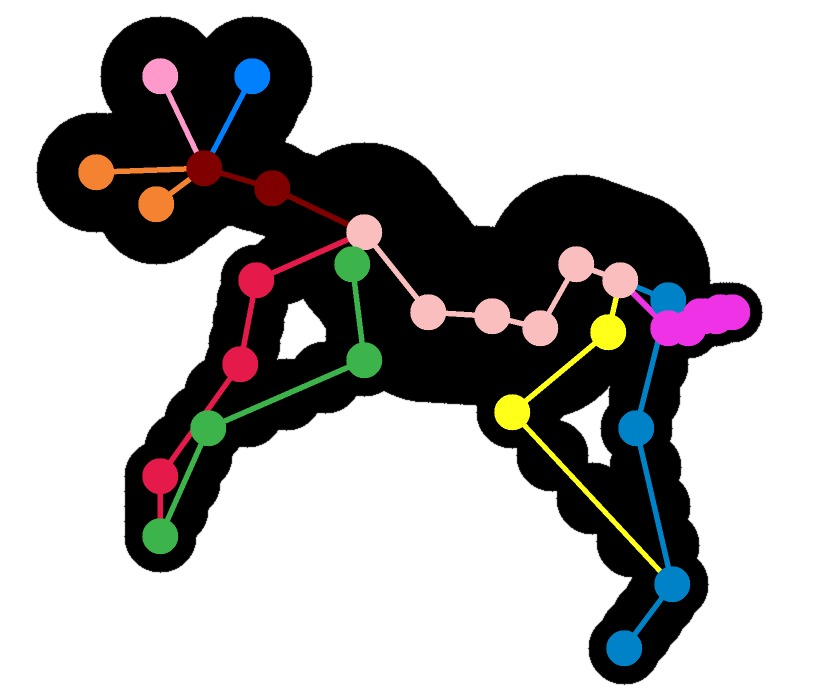
\includegraphics[width=0.49\linewidth]{sil_coverage_new/approx_render_cov_cropped.jpg}}
\scalebox{-1}[1]{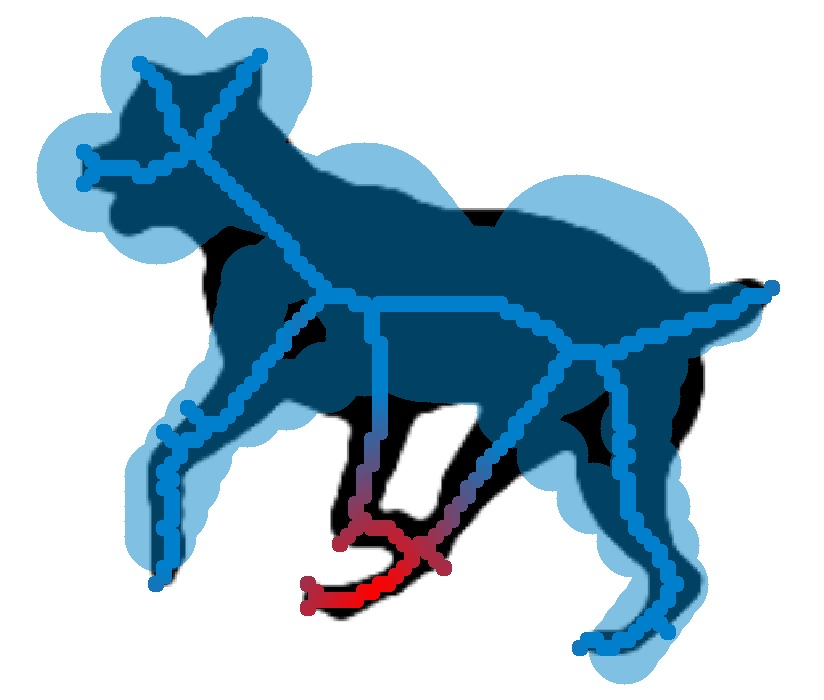
\includegraphics[width=0.49\linewidth]{sil_coverage_new/med_axis_overlay_error_cropped.jpg}}
% predictions taken from rs_dog frame 0100
\end{center}
}
{\caption{Silhouette coverage loss. The error (shown in red) is the the distance between the median axis transform (right) and the nearest point on an approximate rendering (left).}
\label{fig:example_errors}}
\ffigbox{ 
    \raisebox{1 em}{
    \centering
    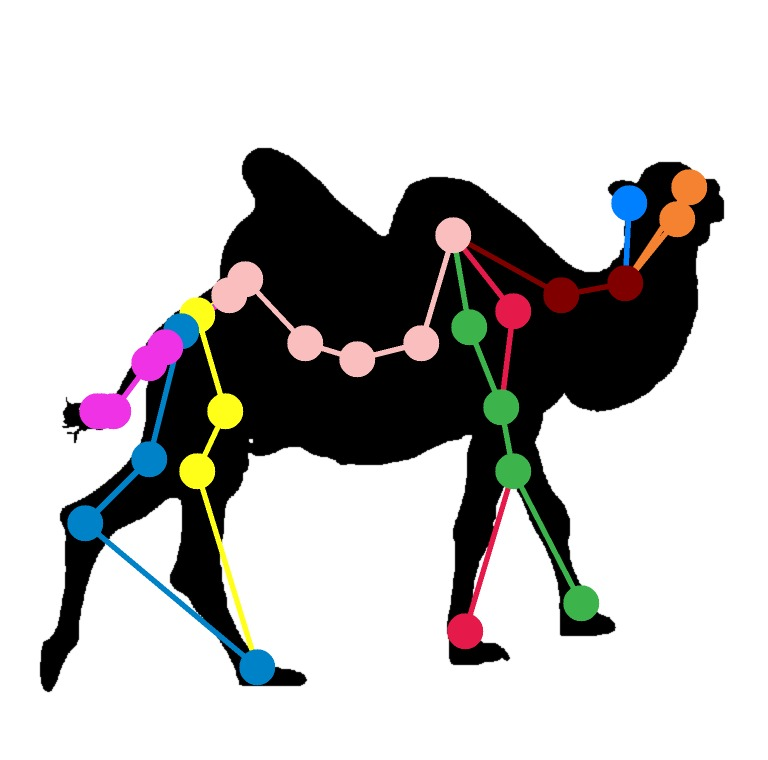
\includegraphics[trim={0cm 0cm 0cm 0cm}, clip,width=0.45\linewidth]{bone_coverage/skeleton_sil_cropped.jpg}
    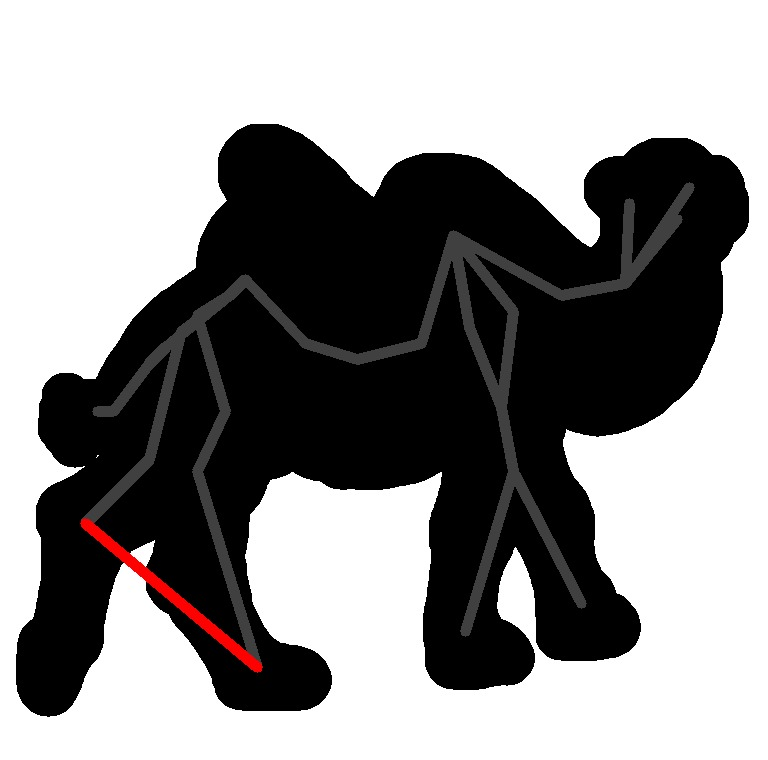
\includegraphics[trim={0cm 0cm 0cm 0cm},clip,width=0.45\linewidth]{bone_coverage/bone_error_overlay_cropped.jpg}
    }
}
{\caption{Bone coverage loss. One of the back-right leg joints is incorrectly assigned (left), leading to a large penalty since the lower leg bone crosses outside the dilated silhouette (right).}
\label{fig:cov-bone}
% camel 0020}
}
\end{floatrow}
\end{figure}

\subsubsection{Bone coverage: $\LL{cov-bone}$}

The bone coverage term is used to prevent bones crossing the background. The joint hierarchy is stored in a kinematic tree structure $K = \{\{j,k\} \text{ if joints } j, k \text{ are connected by a bone}\}$.
\begin{equation}
\LL{cov-bone}(A^{t};X^{t},\silhouette^{t},K) = \sum_{\{j,k\} \in K}\biggl(1 - \min_{\lambda \in \big[0:0.1:1\big]}\silhouette^{t}(\hat{X}_{j}^{t} + \lambda(\hat{X}_{j}^{t} - \hat{X}_{k}^{t}))\biggr)
\end{equation}

\subsection{Formulation as a genetic algorithm}
We minimize this more complex objective using a genetic algorithm (GA)\cite{holland1992adaptation}. A genetic algorithm is a method for solving optimization problems using a natural selection process that mimics biological evolution. Unlike the quadratic program described previously, the GA optimization procedure relies on crossover and mutation, rather than by calculating derivatives. In some cases (and as shown in this work), this can lead to much faster convergence properties. The following components are required:

\ss{Genes.} Candidate solutions to the optimization problem are referred to as a set of `genes'. In this case, a gene is the asssignment array $A$ although is represented as a vector of $J$ integers (indicating the proposal ID), rather than one-hot encodings. 

\ss{Initial population.} Genes are constructed subject to the constraints given in \Cref{eq:quadprog}. The genetic algorithm is initialized with a population size of 128 genes. Of these, the first 32 are set equal to the max confidence solutions given by the network, which speeds up convergence. The remaining 96 genes are generated by selecting a random proposal for each joint. 

\ss{Fitness function.} A fitness function is used to evaluate the quality of a gene. In this setting, the fitness function is precisely the energy $L(A)$ given above which minimizes to yield an optimal skeleton configuration.

\ss{Crossover.} Crossover is a fundemental operation common to evolutionary methods which defines the process of combining the information of two `parent' genes to generate an offspring gene. \emph{Single-point} crossover operates by slicing parent genes each into two parts, and combining first and second parts from different parents to yield the next generation. Following standard practice, the crossover point is randomly selected for each combination. 

\ss{Mutation.} Analogous to biological mutation and used to maintain diversity among genes, each gene is assigned some probability of undergoing a {\em mutation}. If a gene 
is selected for mutation, between 1 and 4 joints have new proposals randomly assigned.

The genetic algorithm described has weights set empirically and is run for 1000 generations. Examples of errors corrected by the additional coverage energy terms are shown in Fig.~\ref{fig:example_errors} and Fig.~\ref{fig:cov-bone}.
